\section{Datenmanagement mit Eigenheiten}

\subsection{Daten}
In diesem Kapitel wird kurz erklärt welche Daten in der Datenbank, sowie in der später erklärten clientraw Dateien verarbeitet werden. Das Weather Display verarbeitet folgende Daten in für Menschen lesbare Produkte:
\begin{itemize}
\item Temperatur
\item Gefühlte Temperatur (Windchill)
\item Maximale, minimale gefühlte Temperatur (Windchill)
\item Gefühlte Temperatur (Hitzeindex)
\item Maximale, minimale gefühlte Temperatur (Hitzeindex)
\item Maximale, minimale Temperatur 
\item Windgeschwindigkeit
\item Maximale Windgeschwindigkeit des Tages 
\item Windrichtung
\item Böengeschwindigkeit
\item Maximale Böengeschwindigkeit des Tages
\item Luftfeuchtigkeit
\item Luftdruck
\item Barometertrend letzte Stunde
\item Regenmenge (täglich, monatlich, jährlich)
\item Regenrate
\item Taupunkt
\item Wolkenhöhe
\item Batteriegstand
\end{itemize}

% ################################
% Datenfluss (Datenbanken, Textfiles und wie alles verknüpft ist)
% ################################
\subsection{Datenfluss}
\textbf{Ist}\\
Damit alle erklärten Vorgänge besser verständlich sind, wurde ein Ablaufdiagramm erstellt mit der heutigen Situation und der zukünftigen erwünschten Situation. Die heutige Situation, braun,  sieht folgendermassen aus. Die Daten werden von der Wetterstation an das Weather-Display gesendet. Dieses verarbeitet die Daten und schreibt sie in eine Textdatei, sowie im Minuten Takt in die Datenbank. Das Weather-Display Live verarbeitet die Daten der Textdatei in eine dynamische Anzeige und erstellt gleichzeitig ein Bild davon. Die Webseite entscheidet dann, ob die dynamische oder die Bild-Anzeige angezeigt wird. Bei der mobilen Webseite wird in jedem Fall vom Bild Gebrauch gemacht. \\
\textbf{Soll}\\
In Zukunft, blau, soll der Datenfluss bis zur Textdatei gleich sein. Anschliessend soll aber ein Javascript Anzeigen von den verarbeiteten Daten erstellen und auf die responsive Webseite angezeigt werden.\\

% Abbildung (A3)
\afterpage{ 
\clearpage
\KOMAoptions{paper=a3, paper=landscape} 
\recalctypearea
\newgeometry{left=30mm,right=30mm,top=30mm,bottom=50mm}

\begin{figure}[h!p]
	\centering
	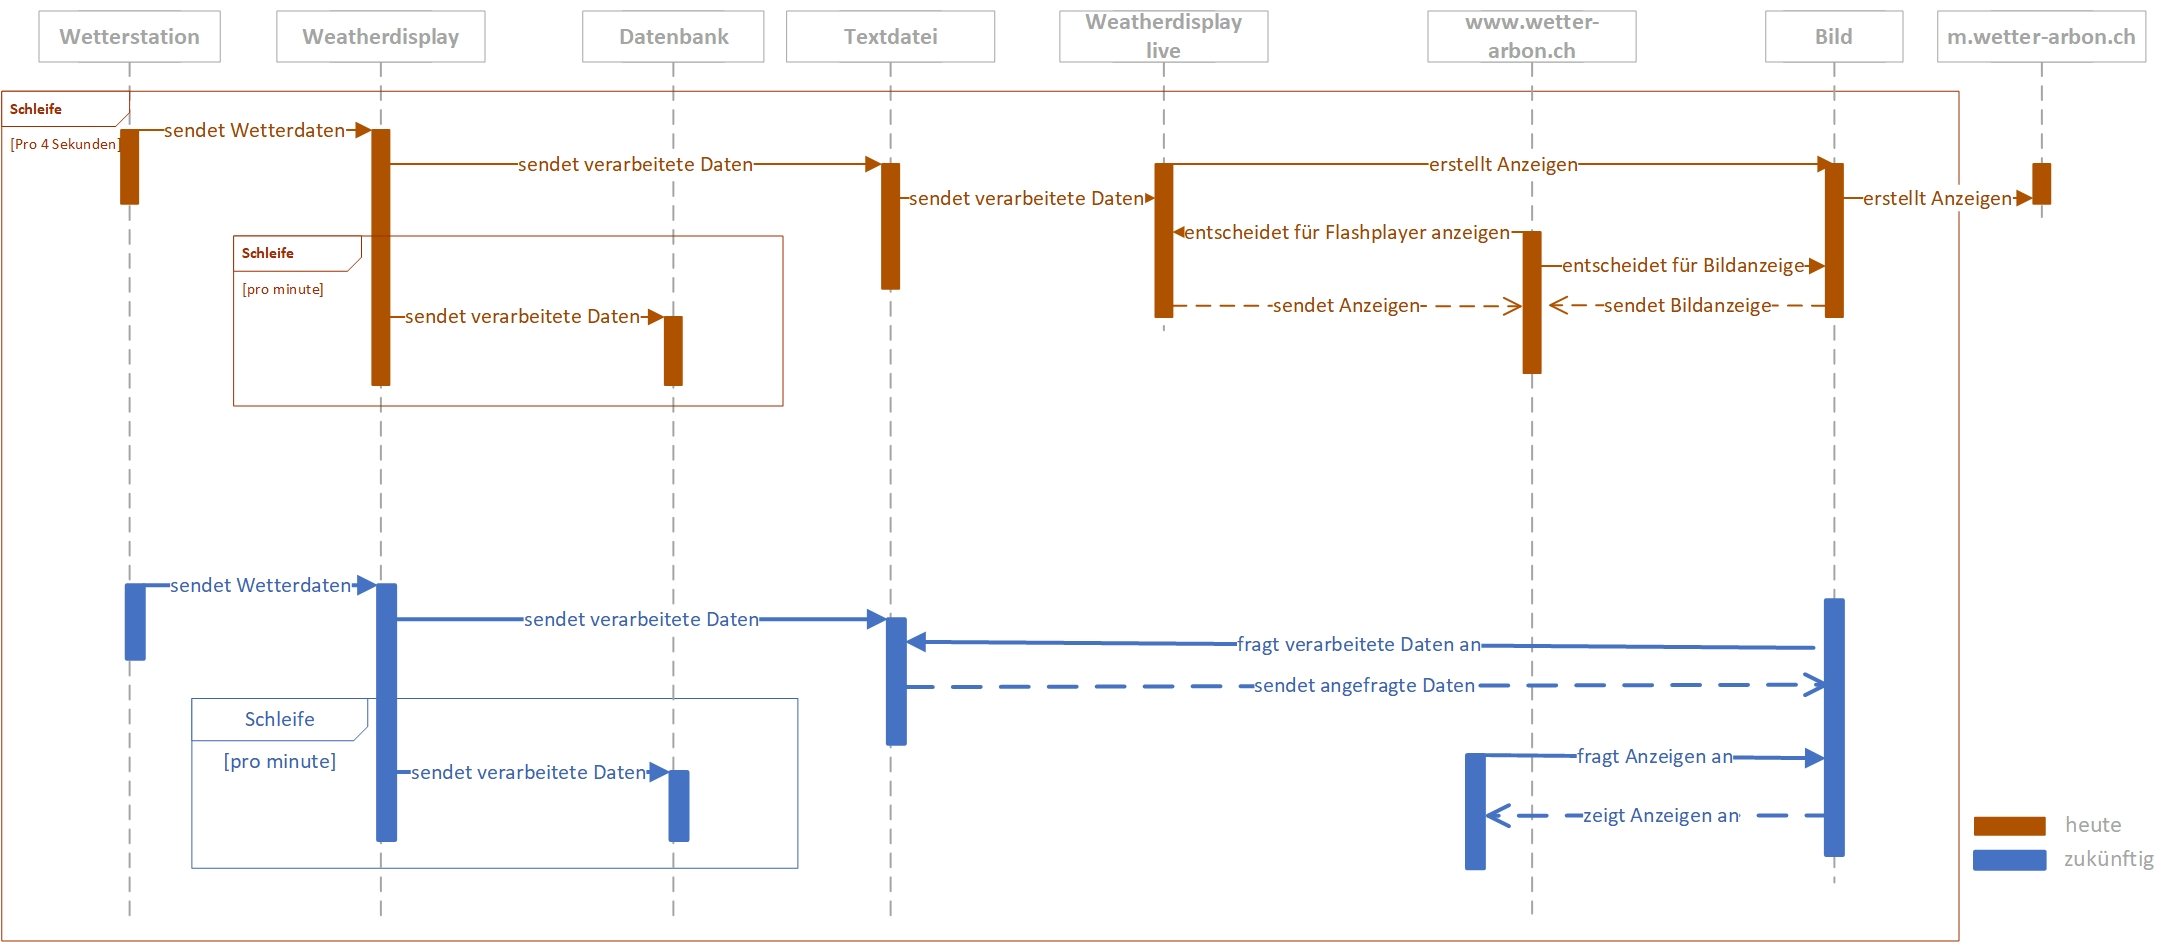
\includegraphics[width=2.5\linewidth]{img/Sequenzdiagramm_Wetter}
	\caption{Ablauf von der Datenerfassung bis zur Anzeige}
	\label{img:Sequenzdiagramm}
\end{figure}


\restoregeometry
\KOMAoptions{paper=A4,pagesize}
\recalctypearea
}




\subsection{Die verschiedenen Datenbanken}
% Datenbanken
\textbf{Ist}\\
Für die Webseite und die Wetterstation, hat es vier verschiedene Datenbanken. Diese werden in diesem Kapitel einzeln behandelt und erklärt wie Sie zusammenhängen bzw. welche Rolle sie für die Webseite spielen. Die vier Datenbanken heissen:
\begin{itemize}  
\item igwetter meteotmpl
\item igwetter wettertest
\item igwetter wp0
\item igwetter openfile64Light
\end{itemize}

Die Datenbank igwetter meteotmpl dient nur als Template und ist nicht in Gebrauch. Dies gilt auch für die igwetter wp0.\\


Die igwetter wettertest dient als Datenspeicher. In der Tabelle wx data sind die Daten ab dem 25.02.2015 bis zum jetzigen Zeitpunkt gespeichert.In der Tabelle tblgestern  sind die täglichen Minimum, sowie Maximas der Daten gespeichert.\\
Für die Applikationen ist die Tabelle applications in der igwetter opfile64Light relevant. Hier werden für die Applikationen die PHP Dateinamen gespeichert. Somit weiss die Webseite wie die Applikation, welche geöffnet werden muss, gespeichert ist.\\



\subsection{Wofür die Text Files benutzt werden}
% Text Files
\textbf{Ist}
Die Weather-Display Software speichert zusätzlich alle Daten, welche von der Wetterstation sind, in ein .txt File. Das Weather-Display live nimmt die Daten direkt aus diesem File um die Anzeigen zu erstellen. Die Daten werden in 4 verschiedenen Textfiles mit unterschiedlichen Funktionen gespeichert.
\begin{itemize}  
\item clientraw.txt
\item clientrawextra.txt
\item clientrawhour.txt
\item clientrawdaily.txt
\end{itemize}


Die clientraw.txt Datei enthält die aktuellen Wetterdaten der Station.  Die clientrawextra.txt enthält die historischen Extremwerte. Die Datei clientrawhour.txt enthält die aufgezeichneten Daten der letzten Stunde im Minutentakt.\cite{WeatherDisplay} 
Die Daten welche in die Datei clientraw.txt geschrieben werden wird in einem gewissen Intervall aktualisiert. Dieser Intervall wird wird in der Konfigurationsdatei wdlconfig.xml eingestellt. Im Fall von Arbon wird die Datei alle 5 Sekunden aktualisiert. Hier werden auch die restlichen Parameter bzw. Einheiten in der die Daten gespeichert werden sollen eingestellt.\\


% ################################
% Datenmanagment und Datensicherung
% ################################
\subsection{Datenmanagement und Datensicherung}
\textbf{Ist}\\
Täglich fallen 93600 Datenpunkte an, diese Daten werden alle seit 2015 gespeichert und nicht ausgedünnt. Wie erwähnt werden nur die igwetter openfile64Light und die igwetter wettertest Datenbank benutzt, für diese beiden Datenbanken gibt es aber kein Backup auf bspw. eine externe Harddisk. Zusätzlich zur Datenbank werden auch die erwähnten clientraw Dateien benutzt um Anzeigen zu erstellen. Von diesen wird jährlich ein Backup erstellt und beim Hosting-service selber gespeichert.\\
\textbf{Problem}\\
Das Problem hierbei ist folgendes schaut man die Datenbanken zum jetzigen Zeitpunkt an, scheint es chaotisch zu sein. Da es aber mehrere Datenbanken gibt,  ist es auf dem ersten Blick nicht sichtbar, was wo gemacht wird und welche Datenbank für wofür zuständig ist.
Das zeigt auch auf wie wichtig eine gute Strukturierung der Datenbank ist.  Ein weiterer Punkt sind die riesigen Mengen an Daten, diese verzögert eine Abfrage in der Datenbank enorm. zum anderen werden die seit dem erstellten Daten nicht auch in die "historische" Tabelle tblgestern abgelegt.


\subsection{Lösungsansatz}
Hierfür wird vorgeschlagen die Datenbank igwetter openfile64Light so zu belassen, da diese für das CMS zuständig ist. Es wird eine neue Datenbank erstellt welche klarer strukturiert wird, hierbei sollten neue Tabellen entstehenen, wobei Daten ausgedünnt werden können um keinen unnötigen Speicherplatz zu belasten. Die Haupttabelle soll alle aktuelle Daten enthalten. Zusätzlich soll Tabelle erstellt werden mit zukünftigen und vorhandenen historischen Daten. Um die Übersichtlichkeit zu gewähren wird eine Tabelle mit Maximal sowie Minimal Daten erstellt. Die Zeitabstände, in der die Daten gelöscht bzw. zu historischen Daten werden, müssen noch mit den Mitgliedern der IG-Wetter abgesprochen werden. Ein weiterer Punkt auf der Liste sollten die zukünftigen Backups sein, d.h. diese sollten nicht als .txt sonder auch als .sql File gespeichert sein damit im Falle eines Datenverlustes die Datenbank einfach wiederherzustellen ist.

% ################################
% API
% ################################
\subsection{API}
\Diskussionspunkt{REST-Service?}

\Diskussionspunkt{API für Badi (Luft- und Wassertemperatur)}

\Diskussionspunkt{Das Kapitel API wurde aus Zeitgründen noch nicht erstellt. Dies wird bis zu definitiven Abgabe noch nachgeholt.}

